\documentclass[First Project.tex]{subfiles}

\begin{document}

\subsection{ Μέθοδος της διχοτόμησης }
Η μέθοδος της διχοτόμησης γενικά προϋποθέτει την ύπαρξη ενός διαστήματος \textlatin{\textbf{[a,b]}} στο οποίο η συνάρτηση έχει τουλάχιστον μία ρίζα. Για να βρούμε ένα 
τέτοιο διάστημα χρησιμοποιούμε το θεώρημα \textlatin{\textbf{Bolzano}} σε συνδυασμό με την γραφική παράσταση της \textlatin{\textbf{f(x)}}. Όπως 
παρατηρούμε στο \textit{Σχήμα 1} η \textlatin{\textbf{f(x)}} έχει μία ρίζα στο διάστημα \textlatin{\textbf{[-1.5,-1.0]}}. Εξάλλου, στο διάστημα 
\textlatin{\textbf{[-1.5,-1.0]}} η \textlatin{\textbf{f(x)}} είναι συνεχής με \[\textlatin{\textbf{f(-1.5)}}*\textlatin{\textbf{f(-1.0)}}<0\] 
συνεπώς σύμφωνα με το θέωρημα \textlatin{\textbf{Bolzano}} έχει μία τουλάχιστον ρίζα στο διάστημα αυτό. Για να βρούμε την ρίζα χρησιμοποιούμε
την συνάρτηση \textit{\textlatin{\textbf{bisection}}} από το αρχείο \textit{\textlatin{\textbf{bisection.py}}} με ορίσματα την συνάρτηση 
\textlatin{\textbf{f(x), a = -1.5, b = -1.0 }}, ενώ το \textlatin{\textbf{default}} όρισμα \textlatin{\textbf{eps}} έχει την τιμή που
χρειάζεται για ακρίβεια \textbf{5} δεκαδικών ψηφίων. H συνάρτηση επιστρέφει την ρίζα της \textlatin{\textbf{f(x)}} στο διάστημα 
\textlatin{\textbf{(a,b)}} και τον αριθμό των επαναλήψεων που χρειάστηκαν για να βρέθει η ρίζα με σφάλμα λιγότερο από \textlatin{\textbf{eps}}.
\vspace{5px}
\begin{figure}[h!]
    \centering
    \captionsetup{justification=centering}
    \begin{center}
        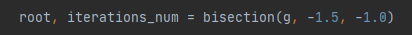
\includegraphics[scale=1]{exercise_1_bisection_call_first_root.png}    
        \caption{Παράδειγμα κλήσης της συνάρτησης \textit{\textlatin{\textbf{bisection}}}}
    \end{center}
\end{figure}

Μετά την κλήση της συνάρτησης \textit{\textlatin{\textbf{bisection}}} τα αποτελέσματα είναι τα εξής:
%\vspace{5px}
\begin{figure}[h!]
    \centering
    \captionsetup{justification=centering}
    \begin{center}
    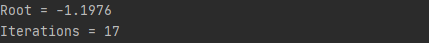
\includegraphics[scale=1]{exercise_1_bisection_results_first_root.png}    
    \caption{ Αποτελέσματα κλήσης της συνάρτησης \textit{\textlatin{\textbf{bisection}}} \\ στο διάστημα \textlatin{\textbf{[-1.5,-1.0]}}. }
    \end{center}
\end{figure}


Ώπου παρατηρούμε ότι η ρίζα της \textlatin{\textbf{f(x)}} στο διάστημα \textlatin{\textbf{[-1.5,-1.0]}} με ακρίβεια 5 δεκαδικών ψηφίων 
είναι η \textbf{-1.1976} καθώς και ότι η μέθοδος της διχοτόμησης χρειάστηκε \textbf{17} επαναλήψεις για να επιτύχει την επιθυμητή ακρίβεια.
Στην συνέχεια παρατηρούμε στο \textit{Σχήμα 1} ότι η \textlatin{\textbf{f(x)}} έχει μία ακόμα ρίζα στο διάστημα \textlatin{\textbf{[1.25,1.75]}}.
Πέρα από την γραφική παράσταση, με παρόμοιο τρόπο χρησιμοποιώντας το θεώρημα \textlatin{\textbf{Bolzano}} μπορούμε να αποδείξουμε ότι η
\textlatin{\textbf{f(x)}} όντως έχει μία τουλάχιστον ρίζα στο διάστημα \textlatin{\textbf{[1.25,1.75]}}. Επομένως καλούμε πάλι την συνάρτηση
\textit{\textlatin{\textbf{bisection}}} αυτή την φορά όμως με ορίσματα \textlatin{\textbf{f(x), a = 1.25, b = 1.75 }}.
\vspace{5px}
\begin{figure}[h!]
    \centering
    \captionsetup{justification=centering}
    \begin{center}
        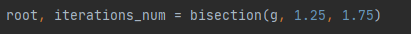
\includegraphics[scale=1]{exercise_1_bisection_call_third_root.png}    
        \caption{Παράδειγμα κλήσης της συνάρτησης \textit{\textlatin{\textbf{bisection}}}}
    \end{center}
\end{figure}

Από την οποία παίρνουμε τα εξής αποτελέσματα:
\begin{figure}[h!]
    \centering
    \captionsetup{justification=centering}
    \begin{center}
    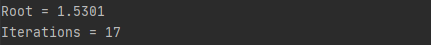
\includegraphics[scale=1]{exercise_1_bisection_results_third_root.png}    
    \caption{ Αποτελέσματα κλήσης της συνάρτησης \textit{\textlatin{\textbf{bisection}}} \\ στο διάστημα \textlatin{\textbf{[1.25,1.75]}}. }
    \end{center}
\end{figure}

Ώπου παρατηρούμε ότι η ρίζα της \textlatin{\textbf{f(x)}} στο διάστημα \textlatin{\textbf{[1.25,1.75]}} με ακρίβεια 5 δεκαδικών ψηφίων 
είναι η \textbf{1.5301} καθώς και ότι η μέθοδος της διχοτόμησης χρειάστηκε \textbf{17} επαναλήψεις για να επιτύχει την επιθυμητή ακρίβεια. 
Τέλος, μπορούμε εύκολα να αποδείξουμε ότι η τρίτη και τελευταία ρίζα της \textlatin{\textbf{f(x)}} είναι το \textbf{0} καθώς 
\textlatin{\textbf{f(0) = 0}}. Στην περίπτωση μας όμως δεν υπάρχει κανένα διάστημα που ταυτόχρονα να περίεχει το \textbf{0} και το θεώρημα
\textlatin{\textbf{Bolzano}} να εγγυάται την ύπαρξη τουλάχιστον μιας ρίζας καθώς δεν υπάρχουν \textbf{\textlatin{x1,x2}} με 
\begin{equation*}
    \textlatin{\textbf{x1}} \neq  \textlatin{\textbf{x2}}, \quad \textlatin{\textbf{x1}},\textlatin{\textbf{x2}} \in \textlatin{\textbf{[-2,2]}} 
\end{equation*}
και
\begin{equation*}
    \textlatin{\textbf{f(x1)}} * \textlatin{\textbf{f(x2)}} < 0 
\end{equation*}
και
\begin{equation*}
    \textbf{0} \in  \textlatin{\textbf{[x1,x2]}} 
\end{equation*}
Συνεπώς η κλασσική μέθοδος της διχοτόμησης δεν εγγυάται σύγκλιση σε αυτή την περίπτωση καθώς και δεν μπορεί να χρησιμοποιηθεί για την εύρεση 
της ρίζας \textbf{\textlatin{x = 0}} αφού προϋποθέτει την ύπαρξη ενός διαστήματος στο οποίο να ισχύει το θεώρημα \textlatin{\textbf{Bolzano}} 
για την \textlatin{\textbf{f(x)}}. Αν προσπαθήσουμε να καλέσουμε την συνάρτηση \textit{\textlatin{\textbf{bisection}}} για ένα διάστημα που
δεν ισχύει το θεώρημα \textlatin{\textbf{Bolzano}} τα αποτελέσματα είναι μη προβλέψιμα και ανάλογα την περίπτωση και τις τιμές του 
διαστήματος \textlatin{\textbf{[a,b]}} η μέθοδος μπορεί να μην συγκλίνει σε σωστή λύση ή να συγκλίνει αλλά όχι με την επιθυμητή ακρίβεια.

\begin{figure}[h!]
    \centering
    \captionsetup{justification=centering}
    \begin{center}
        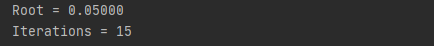
\includegraphics[scale=1]{exercise_1_bisection_results_minus005_005.png}    
        \caption{ Αποτελέσματα κλήσης της συνάρτησης \textit{\textlatin{\textbf{bisection}}} \\ στο διάστημα \textlatin{\textbf{[-0.05,0.05]}}. }
    \end{center}
\end{figure}

\begin{figure}[h!]
    \centering
    \captionsetup{justification=centering}
    \begin{center}
        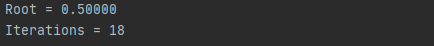
\includegraphics[scale=1]{exercise_1_bisection_results_minus05_05.png}    
        \caption{ Αποτελέσματα κλήσης της συνάρτησης \textit{\textlatin{\textbf{bisection}}} \\ στο διάστημα \textlatin{\textbf{[-0.5,0.5]}}. }
    \end{center}
\end{figure}

Η συνάρτηση \textit{\textlatin{\textbf{bisection}}} που έχει υλοποιηθεί στο αρχείο 
\textit{\textlatin{\textbf{bisection.py}}} ελέγχει αν στο διάστημα \textlatin{\textbf{[a,b]}} ισχύει 
\begin{equation*}
    \textlatin{\textbf{f(x1)}} * \textlatin{\textbf{f(x2)}} > 0
\end{equation*}
και αν ναι επιστρέφει την τιμή \textlatin{\textbf{nan}} ως ρίζα και την τιμή \textbf{-1} ως τον αριθμό των επαναλήψεων. Η συνάρτηση
έχει τροποποιηθεί επίσης ώστε να ελέγχει αν τα άκρα του αρχικού διαστήματος \textlatin{\textbf{[a,b]}} αποτελούν ρίζες της \textlatin{\textbf{f(x)}}.
Αν προσπαθήσουμε τώρα να καλέσουμε την συνάρτηση \textit{\textlatin{\textbf{bisection}}} στην τροποποιημένη μορφή της παρατηρούμε τα εξής:
\vspace{5px}
\begin{figure}[h!]
    \centering
    \captionsetup{justification=centering}
    \begin{center}
        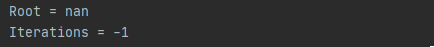
\includegraphics[scale=1]{exercise_1_bisection_results_not_bolzano.png}    
        \caption{ Αποτελέσματα κλήσης της τροποποιήμενης συνάρτησης \textit{\textlatin{\textbf{bisection}}} \\ στο διάστημα \textlatin{\textbf{[-0.5,0.5]}}. }
    \end{center}
\end{figure}
\vspace{5px}
\begin{figure}[h!]
    \centering
    \captionsetup{justification=centering}
    \begin{center}
        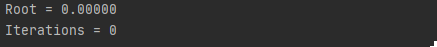
\includegraphics[scale=1]{exercise_1_bisection_results_modified_second_root.png}    
        \caption{ Αποτελέσματα κλήσης της τροποποιήμενης συνάρτησης \textit{\textlatin{\textbf{bisection}}} \\ στο διάστημα \textlatin{\textbf{[0,1]}}. }
    \end{center}
\end{figure}

όπου στην πρώτη κλήση δεν ισχύει το θέωρημα \textlatin{\textbf{Bolzano}} ενώ στην δεύτερη το ένα άκρο του διαστήματος είναι ρίζα της 
\textlatin{\textbf{f(x)}}. Τέλος, τονίζεται ότι αν και τα δύο άκρα του διαστήματος είναι ρίζες της \textlatin{\textbf{f(x)}} επιστρέφεται 
η τιμή του \textlatin{\textbf{a}}.
\newpage

\end{document}
